\chapter{Proiectarea rețelei de profile} \label{chapter:proiectarea}

Proiectarea rețelei de profile se face în cazul nostru pe o secțiune cilindrică în zona dintre periferie și butuc care desparte cele două regiuni în zone de trecere pentru debite de aceeași mărime. Astfel obținem o secțiune prin turbină unde putem practic proiecta geometria pentru o rețea infinită de profile.

\section{Calculul vitezelor}

Considerăm zona de interacțiune a turbinei cu fluidul în trei porțiuni:
\begin{itemize}
	\item prima zonă numită zonă amonte stator ZAS
	\item a doua porțiune: zona stator-rotor numită de acum ZSR
	\item zona trei sau zona aval rotor ZAR
\end{itemize}

La ZAS avem doar viteza axială $V_{a}$ din figura 4.1. care se menține pe toate cele trei porțiuni considerate ale turbinei, iar valoarea acesteia este:

\begin{equation}
V_a=\frac{Q}{\pi(R_{p}^2 - R_{b}^2)} = \frac{0.07}{\pi(0.110^2 - 0.094^2)} = 6.8\si{m/s}
\end{equation}

\begin{figure}[h!]
	\centering
	\includegraphics[scale=0.55]{figures/triunghi_viteza_ZAS.jpg}
	\caption{Viteză în zona aval-stator}
	\label{Viteză în zona aval-stator}
\end{figure}

\subsection{Alegerea razei de calcul a rețelelor}

Pentru proiectarea rețelelor de profile se calculează întâi raza medie a rețelelor la care se vor face în continuare calculele triunghiurilor de viteze. Se alege pentru aceasta o rază medie $R_m$ între raza de periferie și raza de butuc astfel încât debitul dintre cele doua zone să fie egale:

\begin{equation}
\frac{Q}{2} = V_a \pi (R_p^2 - R_m^2) 
\end{equation}

\begin{equation}
V_a \pi (R_p^2 - R_m^2) = 2 V_a \pi (R_p^2 - R_m^2) 
\end{equation}

\begin{equation}
R_p^2 - R_m^2 = 2 R_p^2 - 2 R_m^2
\end{equation}

\begin{equation}
R_m = \sqrt{\frac{R_p^2 + R_b^2}{2}} = \sqrt{\frac{0.110^2 + 0.094^2}{2}} = 0.102\si{m}
\end{equation}

În ZSR, avem viteza tangențială $U$:

\begin{equation}
U = \omega R_m \text{ sau } \frac{\pi n}{30} R_m = \frac{\pi \cdot 1500}{30} 0.102 = 16.0 \si{m/s}
\end{equation}

Conform ecuației fundamentale a turbomașinilor (ecuația lui Euler) avem viteza absolută:

\begin{equation}
gH=UV_{u}, \text{ sau } gH=\frac{\pi n}{30} R_m V_{u}
\end{equation}

\begin{equation}
V_{u} = \frac{30gH}{\pi n R_m} = \frac{30 \cdot 9.81 \cdot 24 }{\pi \cdot 1500 \cdot 0.102} = 14.7 \si{m/s}
\end{equation}


Unghiul $\alpha_2$ dintre direcția tangențială și viteza absolută $V_u$ este:

\begin{equation}
tan(\alpha_{2 })=\frac{V_{u}}{V_{a}} = \frac{14.7}{6.8} \Rightarrow \alpha_{2}=65.1\si{\degree}
\end{equation}


Unghiul $\beta_2$ dintre direcția tangențială și viteza relativă $W_2$ este:

\begin{equation}
tan(\beta_{2})=\frac{V_u - U}{V_a} = \frac{14.7 - 16.0}{6.8} \Rightarrow \beta_{2} = -11.0\si{\degree}
\end{equation}


\section{Triunghiurile de viteză}

Triunghiurile de viteză pentru ZSR se prezintă conform figurii 4.2.:

\begin{figure}[h!]
	\centering
	\includegraphics[scale=0.55]{figures/triunghi_viteza_ZSR.jpg}
	\caption{Triunghi viteză în zona stator-rotor}
	\label{Triunghi viteză în zona stator-rotor}
\end{figure}


Pentru ZAR avem aceeași viteză axială $V_a$ respectiv tangențială $U$. Putem calcula unghiul $\beta_3$ pentru a completa triunghiurile de viteză.

\begin{equation}
tan(\beta_{3})=\frac{-U}{V_a} = \frac{-16.0}{6.8} \Rightarrow \beta_{3} = -66.9\si{\degree}
\end{equation}

\begin{figure}[h]
	\centering
	\includegraphics[scale=0.55]{figures/triunghi_viteza_ZAR.jpg}
	\caption{Triunghi viteză în zona aval rotor}
	\label{Triunghi viteză în zona aval rotor}
\end{figure}

\clearpage

\section{Alegerea pasului rețelei. Criteriul Zweifel}

Conform monografiei \cite[p.102]{hall2013fluid}, pentru paletele de turbină există un raport pas-coarda optim care oferă un minim general de pierderi. Figura 4.4. ilustrează modul în care distribuția vitezelor variază în jurul suprafeței unei palete de turbine așezată în serie la trei valori ale pasului relativ.

\begin{figure}[h]
	\centering
	\includegraphics[scale=0.35]{figures/pasul_relativ_optim.jpg}
	\caption{Pasul relativ optim pentru o turbină \cite{hall2013fluid}}
	\label{Pasul relativ optim pentru o turbină}
\end{figure}

Pentru pas relativ mic, fluidul are un ghidaj maxim, dar pierderile prin frecare vor fi mari. Pe de altă parte, cu aceleași palete așezate la un pas mai mare, pierderile prin frecare sunt mici dar, din cauza ghidării defectuoase a fluidului, pierderile rezultate din separarea curentului sunt ridicate. Datorită acestor considerații, O. Zweifel \cite{zweifel1945frage} a formulat criteriul pentru raportul optim dintre pas și extensia axială a paletei ce au unghiuri mari de deviere.

\begin{figure}[h]
	\centering
	\includegraphics[scale=0.5]{figures/distributia_presiunii.jpg}
	\caption{Distribuție tipică a presiunii pe paleta de turbină \cite{hall2013fluid}}
	\label{Distribuție tipică a presiunii pe paleta de turbină}
\end{figure}

Figura 4.5. indică o distribuție tipică a presiunii într-o rețea de palete în turbină cu fluid incompresibil, curbele $P$ și $S$ corespunzătoare feței de presiune (sau concavă), respectiv depresiune (convexă).

Zweifel a găsit empiric pentru turbine următoarea formulă care depinde de unghiurile de intrare și de ieșire a fluidului în rețea:

\begin{equation}
Z_w = 2 \frac{s}{b} cos^2\alpha_2 (tan\alpha_2 - tan\alpha_1)
\end{equation}

La numere Mach mici, pentru pierderi minime a fost aproximată o valoare a $Z_w = 0.8$, astfel având stabilite unghiurile de intrare și de ieșire putem calcula pasul relativ în următorii pași:

\begin{equation}
0.8 = 2 \frac{s}{b} cos^2\alpha_2 (tan\alpha_1 + tan\alpha_2)
\end{equation}

\begin{equation}
\frac{s}{b} = \frac{0.4}{cos^2\alpha_2 (tan\alpha_1 + tan\alpha_2)}
\end{equation}

\begin{equation}
\frac{s}{b} = 0.4 \frac{1+tan^2\alpha_2}{tan\alpha_1 + tan\alpha_2}
\end{equation}

\begin{equation}
\frac{s}{b} = 0.4 \frac{1 + (V_u / V_a)^2 } {0 + (V_u / V_a)}
\end{equation}

\vspace{5mm} %5mm vertical space

Pentru stator $tan\alpha_1 = 0$ și ajungem la următorul rezultat:

\begin{equation}
(s/b)_{stator} = 0.4 \frac{1 + (14.7 / 6.8)^2 } {0 + (14.7 / 6.8)}\cong 1.05
\end{equation}

\vspace{5mm} %5mm vertical space

Pentru rotor avem următoarea ecuație:

\begin{equation}
\frac{s}{b} = 0.4 \frac{1+tan^2\beta_3}{tan\beta_2 + tan\beta_3}
\end{equation}

\begin{equation}
\frac{s}{b} = 0.4 \frac{1 + (U / V_a)^2 } {(U - V_u) / V_a + (V_u / V_a)}
\end{equation}

\begin{equation}
(s/b)_{rotor} = 0.4 \frac{1 + (16 / 6.8)^2 } {(16 - 14.7) / 6.8 + (14.7 / 6.8)} \cong 1.03
\end{equation}

\clearpage


\section{Proiectare palete}

Proiectarea rețelei de profile se face efectiv proiectând geometria paletelor cunoscând direcțiile de curgere ale fluidului în zona amonte respectiv aval, $tan\alpha_1$ și $tan\alpha_2$ și de asemenea pasul rețelei. Având aceste informații din secțiunile precedente, forma paletelor precum și distribuția de presiune pe palete se determină asumând o vorticitate medie pe pas $dV_u/dx$ variind de la bordul de atac, $x=0$ pana la bordul de fuga $x=1$. Dacă funcția $f_0(x), x \in [0,1]$ denotă liniile de curent pentru un debit mediu în rețea, atunci $f_0'(x)$ este direcția de curgere și $f_0''(x)$ este viteza corespunzătoare, după cum urmează:

\begin{equation}
f_0''(x) = ( tan\alpha_2 - tan\alpha_1 ) g(x),
\end{equation}

\begin{equation}
f_0'(x) = tan\alpha_1 + ( tan\alpha_2 - tan\alpha_1 ) \int_{0}^x g(t)dt,
\end{equation}

\begin{equation}
f_0(x) = x tan\alpha_1 + ( tan\alpha_2 - tan\alpha_1 ) \int_{0}^x \Big( \int_{0}^s g(t)dt \Big) ds.
\end{equation}

Putem defini o funcție unitară normalizată de distribuție a presiunii pe paletă $g(x)$. Cum $f_0"(0) = tan \alpha_1$ si $f_0' = tan \alpha_2$, integrată $g(x)$ de la 0 la 1 este 1. De asemenea, datorită condiției Kutta-Jukowski la bordul de fugă, este obligatoriu ca $g(1) = 0$.

Aceasta abordare se numește \textit{metoda inversa de design} pentru că se definește întâi curgerea și apoi geometria paletelor. Metoda clasica, \textit{metoda directă de design}, optimizează geometria parametrizată a paletei alegând diferite funcții obiective, în cazul nostru alegem parametrii de distribuție a încărcării, $g(x; \lambda_1, \lambda_2,...)$ și determinăm parametrul $\lamba_i$ minimizând viteza maximă de pe paletă, astfel asigurând un comportament cavitațional eficient.

Pentru a putea proiecta paleta începem prin alegerea parametrilor pentru funcția de încărcare:

\begin{equation}
g(x; \lambda_1, \lambda_2, \lambda_3) = erf(\lambda_1 x) \times erf( \lambda_2( 1 - x )) \times (1 + \lambda_3x ).
\end{equation}

\begin{figure}[!h]
  \centering
    \includegraphics[scale=0.5]{figures/loading-shape.PNG}
  \caption{Legea de încărcare pentru stator (stânga) și rotor (dreapta)}
\end{figure}

Cu funcția de încărcare scalata de integrala sa de la 0 la 1.

Procedura de optimizare pentru paleta subțire folosește viteza maximă pe paleta ca funcție obiectiv pentru minimizarea automată a celor trei parametrii din (4.24) cu algoritmul BOBYQA (vezi anexa A.2.5) \cite{powell2009bobyqa} obținând un rezultat conform figurii 4.6.

Integrând consecutiv funcția de încărcare cu cei trei parametrii aleși, obținem funcțiile din figura 4.7, integrala de ordin întâi reprezentând și estimarea inițială a geometriei paletei obținută numeric pe care o putem optimiza în pasul următor.

\begin{figure}[h]
	\centering
	\includegraphics[scale=0.35]{figures/stator_initial_blade.eps}
	\caption{Varianta inițială a geometriei paletei statorului}
	\label{Varianta inițială a geometriei paletei statorului}
\end{figure}

După optimizarea iterativă a formei paletei statorului cu ajutorul programului din anexa A.2.5. obținem rezultatul din figura 4.8. Acești pași se repeta și pentru rotor obținând astfel geometria subțire a acestora, iar în capitolul următor trecem la analiza numerica a rezultatelor obținute în ANSYS Fluent pentru a putea valida rezultatele, urmând ca apoi sa adaugăm și o funcție de grosime pentru profilele subțiri astfel ajungând la un rezultat ce se poate folosi în realitate la o turbina axială de destindere.

\begin{figure}[t]
	\centering
	\includegraphics[scale=0.4]{figures/stator_optimized_blade.eps}
	\caption{Varianta optimizată a geometriei paletei statorului}
	\label{Varianta optimizată a geometriei paletei statorului}
\end{figure}

\clearpage